%%%% Better Poster latex template example v1.0 (2019/04/04)
%%%% GNU General Public License v3.0
%%%% Rafael Bailo
%%%% https://github.com/rafaelbailo/betterposter-latex-template
%%%% 
%%%% Original design from Mike Morrison
%%%% https://twitter.com/mikemorrison

\documentclass[a0paper,fleqn]{betterposter}

%%%% Uncomment the following commands to customise the format

%% Setting the width of columns
% Left column
\setlength{\leftbarwidth}{0.26\paperwidth}
% Right column
\setlength{\rightbarwidth}{0.225\paperwidth}

%% Setting the column margins
% Horizontal margin
%\setlength{\columnmarginvertical}{0.05\paperheight}
% Vertical margin
\setlength{\columnmarginhorizontal}{0.02\paperheight}
% Horizontal margin for the main column
\setlength{\maincolumnmarginvertical}{0.05\paperheight}
% Vertical margin for the main column
%\setlength{\maincolumnmarginhorizontal}{0.15\paperheight}

%% Changing font sizes
% Text font
%\renewcommand{\fontsizestandard}{\fontsize{28}{35} \selectfont}
% Main column font
%\renewcommand{\fontsizemain}{\fontsize{28}{35} \selectfont}
% Title font
\renewcommand{\fontsizetitle}{\fontsize{105}{35} \selectfont}
% Author font
\renewcommand{\fontsizeauthor}{\fontsize{35}{20} \selectfont}
% Section font
%\renewcommand{\fontsizesection}{\fontsize{28}{35} \selectfont}

%% Changing font sizes for a specific text segment
% Place the text inside brackets:
% {\fontsize{28}{35} \selectfont Your text goes here}

%% Changing colours
% Background of side columns
\renewcommand{\columnbackgroundcolor}{lightpurple}
% Font of side columns
%\renewcommand{\columnfontcolor}{gray}
% Background of main column
% \renewcommand{\maincolumnbackgroundcolor}{empirical}
% \renewcommand{\maincolumnbackgroundcolor}{theory}
% \renewcommand{\maincolumnbackgroundcolor}{methods}
% \renewcommand{\maincolumnbackgroundcolor}{intervention}
% Font of main column
%\renewcommand{\maincolumnfontcolor}{gray}

\usepackage{setspace}

\begin{document}
    \betterposter{
    %%%%%%%% MAIN COLUMN
    \maincolumn{
    %%%% Main space
        \vspace{100pt}

        \begin{spacing}{3.5}
            \begin{flushleft}
            {\fontsize{140}{400}\selectfont \textbf{O waste! o waste,}},
            \end{flushleft}
            \vspace{50pt}
            \begin{flushright}
                {\fontsize{140}{10}\selectfont \textbf{wherefore art thou?}}
            \end{flushright}
        \end{spacing}

        \begin{minipage}{0.50\textwidth}
            \begin{spacing}{3}
            \begin{center}
                    {\fontsize{80}{90}\selectfont  \textit{With code our guide,}}
                \vspace{40pt}\\
                {\fontsize{80}{90}\selectfont  \textit{we seek to find,}}
                \vspace{40pt}\\
                {\fontsize{80}{35}\selectfont \textit{hidden hotspots,}}
                \vspace{40pt}\\
                {\fontsize{80}{35}\selectfont \textit{where waste entwined.}}
            \end{center}
            \end{spacing}

            \vspace{200pt}
            \begin{center}
            \begin{spacing}{3}
            {\fontsize{46}{20}\selectfont We created the WasteFootprint tool\\to track supply-chain waste in LCA\\}
            \vspace{10pt}
            \end{spacing}
            \vspace{30pt}
            \end{center}
            \end{minipage}
        \begin{minipage}{0.5\textwidth}
        \begin{flushleft}
            \vspace{220pt}
            
\includegraphics[width=0.9\textwidth]{img/foot.pdf}
        \end{flushleft}
        \vspace{100pt}
        \end{minipage}
        
\includegraphics[height=0.1\textwidth]{img/logoUL_white}\hfill
        
\includegraphics[height=0.07\textwidth]{img/python}\hfill
        
\includegraphics[height=0.07\textwidth]{img/brightway}

    }{
        %%%% Bottom space
        %% This fills the space between the content and the logo
        %% QR code
        %% Institution logo
    }
    }{
    %%%%%%%% LEFT COLUMN

    \title{WasteFootprint}
    {\fontsizesection\selectfont\textbf{a flexible tool for analysing\\ supply-chain waste flows in LCA}}\\

    \author{Elizabeth Lamphere, Stewart Charles McDowall, Stefano Cucurachi \& Carlos Felipe Blanco Rocha}
    \vspace{20pt}
    \institution{CML, Leiden University, The Netherlands}
    {\fontsize{35}{30}\selectfont Presented at the ISIE conference on July 3, 2023}
    
    \section{\hspace{2cm}Why?}\\
    To promote `circularity' we must understand waste, but supply-chain waste in LCA is not well understood as most focus is on downstream waste

    \section{\hspace{2cm}What?}\\
    We've written an extension to the brightway2 LCA framework that calculates the waste footprint of a product or service.
    It finds upstream waste flows in a supply chain, categorises waste flows into 14 types and finds hotspots in waste generation.

    \section{\hspace{2cm}How?}\\
It explodes the database, identifies upstream waste exchanges, edits them and writes custom WasteFootprint methods. The waste flows then become pseudo-biosphere flows and the waste footprint can be calculated as an LCIA method.

    \section{\hspace{2cm}Challenges?}\\
\textbf{Data completeness:} ca. 95\% of waste has no EoL\\
\textbf{Waste is not all the same:} Sometimes `inert-waste' is just moving some rocks around\\
 \textbf{LCA system models:} both attributional and consequential models make a mess of this

    \section{\hspace{2cm}What next?}\\
        The method will be refined and also extended with case studies and ex-ante exploration.\\
        The WasteFootprint tool can be easily applied to calculate the `footprints' of other supply-chain flows
        such as water, gas, and critical raw materials.

    }{
    %%%%%%%% RIGHT COLUMN
    \begin{center}
    {\fontsizesection\selectfont \textbf{         Step by step through the code}}\\
    \vspace{30pt}    
    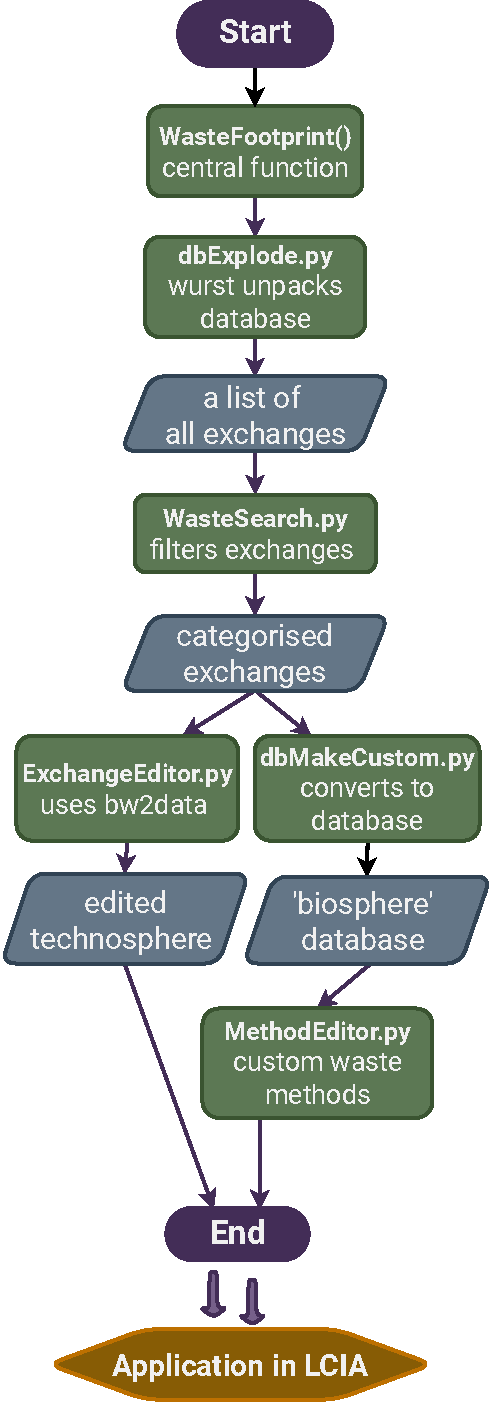
\includegraphics[width=1\textwidth]{img/Flowchart_WasteFootprint.pdf}\\
    \vspace{30pt}
    {\fontsize{36}{40}\selectfont View the WasteFootprint code\\ in our GitHub repository\\}
    \vspace{10pt}
    
\includegraphics[width=0.3\textwidth]{img/qr-code.pdf}
    \end{center}
}

\end{document}

